\documentclass{article}
\usepackage[utf8]{inputenc}
\usepackage[icelandic]{babel}
\usepackage[T1]{fontenc}
\usepackage{graphicx}
\usepackage{mathtools}
\usepackage{amsmath}
\usepackage{amssymb}
\usepackage{minted}
\usepackage{listings}
\usepackage{color}

\definecolor{dkgreen}{rgb}{0,0.6,0}
\definecolor{gray}{rgb}{0.5,0.5,0.5}
\definecolor{mauve}{rgb}{0.58,0,0.82}

\lstset{frame=tb,
  language=Java,
  aboveskip=3mm,
  belowskip=3mm,
  showstringspaces=false,
  columns=flexible,
  basicstyle={\small\ttfamily},
  numbers=none,
  numberstyle=\tiny\color{gray},
  keywordstyle=\color{blue},
  commentstyle=\color{dkgreen},
  stringstyle=\color{mauve},
  breaklines=true,
  breakatwhitespace=true,
  tabsize=3
}

\graphicspath{ {./} }
\title{Vikublað 10 - tölvunarfræði 2}
\author{ttb3@hi.is}
\date{\today}


\begin{document}
\maketitle

\section*{4.1.14}
BFS notar \emph{queue} til að geyma upplýsingar um hnúta sem búið er að skoða.
Þetta gerir BFS kleift að finna stysta veg á milli tveggja hnúta.
Ef við myndum nota \emph{stack} myndi það hafa áhrif á leitina á þann hátt að öll önnur hliðin væri farin áður en byrjað væri að skoða hina.
Frekar illa orðað en sjá teikningar,
\begin{center}
    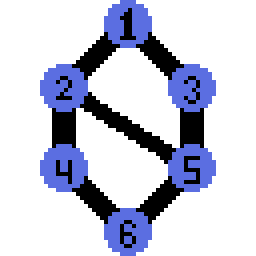
\includegraphics{graph.png}
\end{center}
Ef við byrjum með þetta tré og förum snöggt í gegnum það hvernig leitað væri í því með BFS þar sem er notað \emph{queue}.
Q táknar queue, P táknar print. Hver lína felur í sér að prenta næsta hnút í röðinni og setja tengda hnúta í röðina. Við byrjum á 1.\\
\begin{center}
    \begin{tabular}{|l|l|}
        \hline
        P&Q\\
        \hline
                    &1\\
                    \hline
        1           &2,3\\
        \hline
        1,2         &3,4,5\\
        \hline
        1,2,3       &4,5\\
        \hline
        1,2,3,4     &5,6\\
        \hline
        1,2,3,4,5   &6\\
        \hline
        1,2,3,4,5,6 &\\
        \hline
    \end{tabular}
\end{center}

Sjáið núna muninn ef við notum \emph{stack} en ekki \emph{queue}:
\begin{center}
    \begin{tabular}{|l|l|}
        \hline
        P&Q\\
        \hline
        &1\\
        \hline
        1&2,3\\
        \hline
        1,3&2,5\\
        \hline
        1,3,5&2,6\\
        \hline
        1,3,5,6&2,4\\
        \hline
        1,3,5,6,4&2\\
        \hline
        1,3,5,6,4,2&\\
        \hline
    \end{tabular}
\end{center}
Sama niðurstaða og við fengjum með DFS, þannig tldr. ef við notum \emph{stack} í stað \emph{queue} í BFS er ekki hægt að fá stystu leið því við erum í raun bara að nota DFS.

\section*{Bacon Tala}
Forritið sem ég gerði notast við DegreesOfSeperation forritið sem gefið er í bókinni. Það skilar veginum auk Bacon tölunar, hér eru Bacon tölur allra leikaranna í Glengarry Glen Ross:
\begin{center}
    \begin{tabular}{|c|c|}
        \hline
        Leikari&Bacon Tala\\
        \hline
        Al Pacino&2\\
        \hline
        Jack Lemmon&1\\
        \hline
        Alec Baldwin&1\\
        \hline
        Ed Harris&1\\
        \hline
        Kevin Spacey&2\\
        \hline
        Alan Arkin&2\\
        \hline
        Jonathan Pryce&2\\
        \hline
        Jude Ciccolella&2\\
        \hline
        Lori Tan Chinn&2\\
        \hline
        Bruce Altman&2\\
        \hline
        Leigh French&2\\
        \hline
        George Cheung&2\\
        \hline
        Neal Jones&2\\
        \hline
        Murphy Dunne&2\\
        \hline
        Dana Lee&2\\
        \hline
        Gregory Snegoff&2\\
        \hline
        Julie Payne&2\\
        \hline
        Diane Dreyer&2\\
        \hline
        Paul Butler&1\\
        \hline
    \end{tabular}
\end{center}

\newpage
\section*{BaconHistogram}
\begin{lstlisting}
    import edu.princeton.cs.algs4.*;

public class BaconHistogram {
    public static void main(String[] args) {
        String filename  = args[0];
        String delimiter = args[1];
        String source    = args[2];

        SymbolGraph sg = new SymbolGraph(filename, delimiter);
        Graph G = sg.graph();
        if (!sg.contains(source)) {
            StdOut.println(source + " not in database.");
            return;
        }

        // run breadth-first search from s
        int s = sg.indexOf(source);
        BreadthFirstPaths bfs = new BreadthFirstPaths(G, s);


        // compute histogram of Kevin Bacon numbers - 100 for infinity
        int MAX_BACON = 100;
        int[] hist = new int[MAX_BACON + 1];
        for (int v = 0; v < G.V(); v++) {
            int bacon = Math.min(MAX_BACON, bfs.distTo(v));
            hist[bacon]++;

            // to print actors and movies with large bacon numbers
            if (bacon/2 >= 7 && bacon < MAX_BACON)
                StdOut.printf("%d %s\n", bacon/2, sg.nameOf(v));
        }

        // print out histogram - even indices are actors
        for (int i = 0; i < MAX_BACON; i += 2) {
            if (hist[i] == 0) break;
            StdOut.printf("%3d %8d\n", i/2, hist[i]);
        }
        StdOut.printf("Inf %8d\n", hist[MAX_BACON]);
    }
}
\end{lstlisting}

\begin{tabular}{|l|r|}
    \hline
    B-Tala  &Fjöldi \\
    \hline
    0       &1      \\
    \hline
    1       &1324   \\
    \hline
    2       &70717  \\
    \hline
    3       &40862  \\
    \hline
    4       &1591   \\
    \hline
    5       &125    \\
    \hline
    ÓE      &655    \\
    \hline
\end{tabular}


\end{document}